\documentclass[nobib]{tufte-handout}

\title{Föreläsning 10: Slumpvariabler $\cdot$ 1MA020}

\author[Vilhelm Agdur]{Vilhelm Agdur\thanks{\href{mailto:vilhelm.agdur@math.uu.se}{\nolinkurl{vilhelm.agdur@math.uu.se}}}}

\date{27 februari 2023}


%\geometry{showframe} % display margins for debugging page layout

\usepackage{graphicx} % allow embedded images
  \setkeys{Gin}{width=\linewidth,totalheight=\textheight,keepaspectratio}
  \graphicspath{{graphics/}} % set of paths to search for images
\usepackage{amsmath}  % extended mathematics
\usepackage{booktabs} % book-quality tables
\usepackage{units}    % non-stacked fractions and better unit spacing
\usepackage{multicol} % multiple column layout facilities
\usepackage{lipsum}   % filler text
\usepackage{fancyvrb} % extended verbatim environments
  \fvset{fontsize=\normalsize}% default font size for fancy-verbatim environments

\usepackage{color,soul} % Highlights for text


\include{mathcommands.extratex}

\begin{document}

\definecolor{darkgreen}{rgb}{0.0627, 0.4588, 0.1451}

\maketitle% this prints the handout title, author, and date

\begin{abstract}
\noindent
Vi fortsätter att diskutera diskret sannolikhetsteori, och introducerar slumpvariabler och deras väntevärden.

Vi använder den teori vi byggt upp för att bevisa några fler resultat inom kombinatoriken.
\end{abstract}

\section{Slumpvariabler}

Hittills är vad vi har sett bara hälften av vad man intuitivt tänker ingår i sannolikhetsteorin -- vi har diskuterat slumpmässiga \emph{händelser}, som antingen inträffar eller inte, men vi har inte definierat slumpmässiga tal. Frågan om ifall det kommer att regna imorgon eller inte kan vi modellera i vår formalism, men inte frågan om hur många millimeter det kommer regna.

\begin{definition}
    Givet ett sannolikhetsrum $(\Omega, \mu)$ är en \emph{slumpvariabel} $X$ som tar värden i $V$ en funktion $X: \Omega \to V$. Givet varje utfall tar alltså vår slumpvariabel ett visst värde, och givet varje\sidenote[][]{Detta är lite av en lögn i det allmänna fallet, eftersom det kan finnas \emph{väldigt} skumma delmängder till $V$, men så länge vi tänker oss våra diskreta sannolikhetsrum är det sant.} delmängd $A\subseteq V$ blir $X\in A$ en händelse -- specifikt är det händelsen
    $$\left\{\omega \in \Omega \given X(\omega) \in A\right\} = X^{-1}(A).$$
\end{definition}

Det allra vanligaste fallet är när $V = \R$ eller någon delmängd till $\R$. I många introtexter om sannolikhetsteori \emph{definierar} man att slumpvariabler tar värden i $\R$ -- men eftersom vi sysslar med kombinatorik kommer vi att vilja ha mer exotiska slumpvariabler, som slumpmässiga permutationer eller slumpmässiga mängder.

\begin{example}
    Låt oss återbesöka vårt exempel med ett tärningskast. Vi konstaterade att vi kan ta $\Omega = \{1,2,3,4,5,6\}$ och $\mu(\omega) = 1/6$ för alla $\omega \in \Omega$.

    Vi kan naturligt betrakta vårt tärningskast som en slumpvariabel -- i detta fall blir det en mycket enkel funktion, $X: \Omega \hookrightarrow \R$ skickar helt enkelt varje $\omega$ på sig självt.
\end{example}

Vårt tärningskast är ett specialfall av ett mer allmänt fenomen, som det kommer vara bekvämt att ha en terminologi för.

\begin{definition}
    Givet en ändlig mängd $V$ är ett \emph{likformigt fördelat slumpmässigt element av $V$} en slumpvariabel $X$ sådan att $\Prob{X = v} = \frac{1}{\abs{V}}$ för varje $v\in V$.\sidenote[][]{Vill man göra detta fullständigt rigoröst i vår formalism kan man säga att $X$ är definierad på sannolikhetsrummet $(V, \mu)$ där $\mu(v) = \frac{1}{\abs{V}}$ för alla $v\in V$, och $X: V \to V$ är identitetsfunktionen.
    
    Men det blir väldigt många abstrakta ord för att inte säga så mycket alls som vi inte redan sade när vi definierade $X$ som att den blir lika med varje element i $V$ med samma sannolikhet.} Alla element av $V$ är alltså lika sannolika. Vi kan skriva detta som
    $$X \uniformIn V.$$

    Detta innebär alltså att för varje mängd $W \subseteq V$ så blir
    $$\Prob{X \in W} = \frac{\abs{W}}{\abs{V}}.$$

    Om någon säger att ``vi låter $X$ vara en slumpmässig graf / träd / mängd / etc.'' utan att specificera hur $X$ är fördelad menar de att den är likformig.
\end{definition}

Vi vet att om vi slår vår tärning många gånger kommer vi i genomsnitt att få upp $3.5$. Hur gör vi den intuitionen rigorös?

\begin{definition}
    \emph{Väntevärdet} av en slumpvariabel $X$ som tar värden i $\R$ ges av\sidenote[][-2.5cm]{Notera att detta är en summa över \emph{alla värden som $X$ kan tänkas ta} -- eftersom vi antagit att $\Omega$ är ändligt eller uppräkneligt så kommer detta vara en summa över ändligt eller uppräkneligt många summander, vilket är okej.
    
    Hade vi velat modellera en \emph{kontinuerlig} slumpvariabel -- som till exempel en normalfördelning, som nog många sett redan -- som kan ta vilket reellt tal som helst som värde, hade vi behövt definiera detta som en integral, inte en summa. Att slippa ge definitioner som fungerar i dessa fall är en av anledningarna till varför vi begränsar oss till bara diskret sannolikhetsteori.}
    $$\E{X} = \sum_{x \in X(\Omega)} x \Prob{X = x}.$$

    Vi tar alltså summan över alla tänkbara värden $x$ för $X$, multiplicerar $x$ med sannolikheten att $X$ faktiskt blir $x$,\sidenote[][0.2cm]{Notera att när den här summan löper över oändligt många tal är det fullt möjligt att den inte konvergerar, trots att $\sum_{x \in X(\Omega)} \Prob{x = X} = 1$. Det finns slumpvariabler som alltid tar ändliga värden, men ändå har oändligt väntevärde.} och summerar. I specialfallet där $X$ bara tar värden $0, 1, 2, \ldots$ blir alltså formeln
    $$\E{X} = \sum_{k=0}^{\infty} k\Prob{X = k}.$$
\end{definition}

\begin{example}
    Så om vi åter tar exemplet med tärningskastet så blir alltså väntevärdet
    \begin{align*}
        \E{X} &= 1\Prob{X = 1} + 2\Prob{X = 2} + \ldots + 6\Prob{X = 6}\\
        &= \frac{1 + 2 + 3 + 4 + 5 + 6}{6} = \frac{7}{3} = 3.5
    \end{align*}
    precis som vi förväntade oss.
\end{example}

Ibland är det mer användbart att skriva definitionen av väntevärde på en alternativ form:

\begin{lemma}\label{lemma_expectation_as_sum_over_omegas}
    Det gäller att\sidenote[][]{Det här fungerar bara för att vi har antagit att våra sannolikhetsrum är ändliga eller uppräkneligt oändliga, så vi kan skriva våra sannolikheter som summor. I det mer allmänna fallet hade vi behövt skriva en integral mot sannolikhetsmåttet, och det kräver betydligt mer avancerad analys än vad vi kan.}
    $$\E{X} = \sum_{\omega \in \Omega} X(\omega)\mu(\omega).$$

    \begin{proof}
        Vi kan skriva
        \begin{align*}
            \E{X} &= \sum_{x \in X(\Omega)} x \Prob{X = x}\\
            &= \sum_{x \in X(\Omega)} x\left(\sum_{\omega \in \Omega: X(\omega) = x} \mu(\omega)\right)\\
            &= \sum_{x \in X(\Omega)} \sum_{\omega \in \Omega: X(\omega) = x} x\mu(\omega)\\
            &= \sum_{x \in X(\Omega)} \sum_{\omega \in \Omega: X(\omega) = x} X(\omega)\mu(\omega)\\
            &= \sum_{\omega \in \Omega} X(\omega)\mu(\omega).
        \end{align*}
    \end{proof}
\end{lemma}

Eftersom vi definierat slumpvariabler som att de helt enkelt är funktioner från $\Omega$ kan vi göra all den algebra vi vanligen kan på funktioner in i $\R$. Till exempel är det, givet två slumpvariabler $X$ och $Y$, helt väldefinierat att skriva $X + Y$, och det betyder precis vad vi förväntar oss att det skall betyda -- vi slumpar ett $X$ och ett $Y$ och sedan adderar vi dem med varandra.

När vi nu har introducerat addition av slumpvariabler så kan vi bevisa vad som, i min mening, är en av de allra mest användbara satserna i hela matematiken.\sidenote[][-0.8cm]{Jag är så klart oerhört partisk, eftersom just gränslandet mellan kombinatorik och sannolikhetsteori är mitt område -- men det är onekligen ett otroligt användbart resultat.}

\begin{lemma}[Väntevärdets linjäritet]
    Givet två slumpvariabler $X$ och $Y$ och två reella tal $a$ och $b$ gäller det att
    $$\E{aX + bY} = a\E{X} + b\E{Y}.$$

    Väntevärdet är alltså linjärt, som funktion från rummet av slumpvariabler in i $\R$.\sidenote[][-1cm]{Detta sätt att formulera det skrapar lite på ytan av en väldigt djup teori -- väntevärden är nämligen ``bara'' integraler mot sannolikhetsmått, och samlingen av funktioner från $\Omega$ in i $\R$ blir ju ett vektorrum. Vi kan ge det vektorrummet en inre produkt genom att skriva $\langle X,Y\rangle = \E{XY}$, och vi har börjat med funktionalanalys.
    
    Men detta är ju en kurs i kombinatorik, så att utforska detta får vänta till en framtida kurs för er.}

    \begin{proof}
        Vi använder den alternativa formeln för väntevärde vi fann i Lemma \ref{lemma_expectation_as_sum_over_omegas} och skriver
        \begin{align*}
            \E{aX + bY} &= \sum_{\omega \in \Omega} (aX + bY)(\omega)\mu(\omega)\\
            &= \sum_{\omega \in \Omega} (aX(\omega) + bY(\omega))\mu(\omega)\\
            &= a\sum_{\omega \in \Omega} X(\omega)\mu(\omega) + b\sum_{\omega \in \Omega} Y(\omega)\mu(\omega)\\
            &= a\E{X} + b\E{Y}.
        \end{align*}
    \end{proof}
\end{lemma}

För att göra det här verkligt användbart behöver vi konceptet med indikatorvariabler, som vi introducerade när vi bevisade inklusion-exklusion.

\begin{proposition}
    För en händelse $A$ blir dess indikatorfunktion $\indSet{A}$, som ges av att $\indSet{A}(\omega) = 1$ om $\omega \in A$ och noll annars, en slumpvariabel.\sidenote[][]{Det är ju en funktion från utfall till reella tal -- per definition är det en slumpvariabel. Vi behöver bara känna igen att den är det.}

    Det gäller att
    $$\Prob{A} = \E{\indSet{A}}.$$

    \begin{proof}
        Per definition har vi att
        \begin{align*}
            \E{\indSet{A}} &= 0\cdot\Prob{\indSet{A} = 0} + 1\cdot\Prob{\indSet{A} = 1}\\
            &= \sum_{\omega: \indSet{A}(\omega) = 1} \mu(\omega)\\
            &= \sum_{\omega \in A} \mu(\omega) = \Prob{A}.
        \end{align*}
    \end{proof}
\end{proposition}

\section{Sperners lemma}

Låt oss nu ta vad vi har lärt oss och tillämpa det på ett faktiskt kombinatoriskt resultat.

\begin{definition}
    En följd av icketomma delmängder
    $$F_1 \subsetneq \ldots \subsetneq F_{k-1} \subsetneq F_k \subseteq [n]$$
    till $[n]$ kallas för en \emph{kedja}. Ifall $k=n$ kallar vi kedjan för en \emph{maximal} kedja,\sidenote[][]{Att vi inte kan ha en längre kedja torde vara uppenbart.} och då måste vi, eftersom vi kräver att varje mängd är en \emph{strikt} delmängd till nästa, ha att $\abs{F_i} = i$. I så fall låter vi också $F_0 = \emptyset$.

    En samling $\mathcal{G}$ av delmängder till $[n]$ kallas för en \emph{anti-kedja} ifall det för varje par $F, G \in \mathcal{G}$ varken gäller att $F \subseteq G$ eller $G \subseteq F$.
\end{definition}

Att varje maximal kedja består av precis $n$ stycken mängder är uppenbart. Hur stor kan en anti-kedja vara? Ett enkelt sätt att skapa sig en sådan är att ta alla delmängder av storlek $k$ till $[n]$ för något $k$ -- att dessa inte kan vara delmängder till varandra är uppenbart. Att det val av $k$ som gör denna anti-kedja som störst blir $\floor{\frac{n}{2}}$ är inte allt för svårt att se.\sidenote[][]{Vi hade också kunnat välja $\ceil{\frac{n}{2}}$, det ger samma storlek.} Är det möjligt att hitta en ännu större genom att ha med delmängder av olika storlekar? Sperners lemma säger oss att svaret är nej.

\begin{lemma}[Sperners lemma]
    För varje anti-kedja $\mathcal{F}$ i $[n]$ gäller det att
    $$\abs{\mathcal{F}} \leq \binom{n}{\floor{\frac{n}{2}}}.$$

    \begin{proof}
        Vi tar en likformigt slumpmässig maximal kedja
        $$\emptyset = F_0 \subsetneq F_1 \subsetneq \ldots \subsetneq F_{n-1} \subsetneq F_n = [n],$$
        och låter $I$ vara mängden av $i$ sådana att $F_i$ ligger i vår anti-kedja $\mathcal{F}$.

        Det är enkelt att se att $I$ innehåller antingen noll eller ett element -- en kedja och en anti-kedja kan ju omöjligen skära varandra i mer än en mängd.\sidenote[][]{Ifall vi hade både $i$ och $j$ i $I$, med $i < j$, hade vi ju haft att $F_i \subsetneq F_j$ med bägge i $\mathcal{F}$, vilket motsäger att $\mathcal{F}$ skulle vara en anti-kedja.}

        Låt oss nu studera slumpvariabeln $X = \abs{I}$. Att vi vet att $I$ bara kan ha noll eller ett element ger oss omedelbart att $\E{X} \leq 1$,\sidenote[][]{Detta kan vi göra till ett allmänt lemma:
            \begin{lemma}
                Om $X(\omega) \leq C$ för varje $\omega \in \Omega$ gäller det att $\E{X} \leq C$.
                \begin{proof}
                    Vi kan räkna
                    \begin{align*}
                        \E{X} &= \sum_{\omega \in \Omega} X(\omega)\mu(\omega)\\
                        &\leq \sum_{\omega \in \Omega} C\mu(\omega)\\
                        &= C\sum_{\omega \in \Omega} \mu(\omega) = C.
                    \end{align*}
                \end{proof}
            \end{lemma}
        } men låt oss studera detta väntevärde också på ett annat sätt.

        Vi kan räkna med hjälp av väntevärdets linjäritet att\sidenote[][]{Här använder vi den kortare notationen $\ind{i \in I}$ för att beteckna $\ind{\omega \in \Omega: i \in I(\omega)}$.}
        \begin{align*}
            \E{X} = \E{\abs{I}} &= \E{\sum_{i=1}^{n} \ind{i \in I}}\\
            &= \sum_{i=1}^{n} \E{\ind{i \in I}} = \sum_{i=1}^{n} \Prob{i \in I}.
        \end{align*}

        Vad är sannolikheten att $i$ ligger i $I$? Att $i$ ligger i $I$ betyder att $F_i \in \mathcal{G}$, per definition. Så vad vi behöver förstå är den slumpmässiga mängden $F_i$.

        Eftersom vi valde vår kedja som en likformigt slumpmässig kedja finns det ingen anledning till varför något tal skulle vara mer sannolikt än något annat att dyka upp i denna mängd. Så $F_i$ är alltså, av symmetriskäl, ett likformigt slumpmässigt element ur $\binom{[n]}{i}$, mängden av delmängder av storlek $i$.

        Vad är sannolikheten att $F_i$ faller i $\mathcal{G}$? Jo, om vi låter $\mathcal{G}_i$ beteckna samlingen av element i $\mathcal{G}$ av storlek $i$ vet vi att $\mathcal{G}_i \subseteq \binom{[n]}{i}$  och $F_i \uniformIn \binom{[n]}{i}$, så vi måste ha att
        $$\Prob{F_i \in \mathcal{G}_i} = \frac{\abs{\mathcal{G}_i}}{\binom{n}{i}}.$$

        Så samlar vi ihop vad vi har listat ut hittills i ett enda uttryck, och använder olikheten\sidenote[][]{Vi har strikt sett inte faktiskt bevisat den någon gång, men det bör vara någorlunda enkelt att övertyga sig själv om att den är sann.} $\binom{n}{i} \leq \binom{n}{\floor{\frac{n}{2}}}$ för alla $i$, har vi att
        $$1 \geq \E{X} = \sum_{i=1}^{n} \Prob{i \in I} = \sum_{i=1}^{n} \frac{\abs{\mathcal{G}_i}}{\binom{n}{i}} \geq \sum_{i=1}^{n} \frac{\abs{\mathcal{G}_i}}{\binom{n}{\floor{\frac{n}{2}}}}$$
        så multiplicerar vi bägge sidorna av detta med $\binom{n}{\floor{\frac{n}{2}}}$ får vi att
        $$\binom{n}{\floor{\frac{n}{2}}} \geq \sum_{i=1}^{n} \abs{\mathcal{G}_i} = \abs{\mathcal{G}}$$
        vilket är precis Sperners lemma, som vi ville bevisa.
    \end{proof}
\end{lemma}

\section{Caro-Weis sats}

Antag att vi har en grupp av $n$ personer på ett läger, och säg att person nummer $i$ känner $d_i$ andra personer sedan tidigare. Du vill bilda en mindre grupp av personer för en lära-känna-varandra-lek\sidenote[][]{Eftersom du är en fruktansvärt ondskefull person. Ingen tycker om sådana lekar.}, så du vill hitta en så stor grupp som möjligt av personer som \emph{inte} känner varandra. Finns det någon garanti för hur stor du kan göra den mindre gruppen?

Den matematiska formaliseringen av det här är så klart i termer av grafer, så låt oss ge de rätta definitionerna först innan vi ger resultatet.

\begin{definition}
    \emph{Graden} av en nod $v$ i en graf $G = (V_G, E_G)$ är antalet kanter noden har. Alltså
    $$d_v = \abs{\left\{e \in E_G \given v \in e\right\}}.$$
\end{definition}

\begin{definition}
    En \emph{oberoende mängd} $S \subseteq V_G$ i en graf $G = (V_G, E_G)$ är en mängd av noder sådana att det inte finns några kanter mellan något par av noder i $S$. Alltså, mängden
    $$E(S) = \left\{\{u,v\} \in E_G \given u, v \in S\right\}$$
    är tom.
\end{definition}

\begin{theorem}[Caro-Wei]
    Varje graf $G$ på $n$ noder, där nod $i$ har grad $d_i$, har alltid en oberoende mängd $S$ sådan att
    $$\abs{S} \geq \sum_{i=1}^{n} \frac{1}{d_i + 1}.$$

    \begin{proof}
        Numrera noderna i $G$ från $1$ till $n$, och välj sedan likformigt slumpmässigt ett nytt sätt att etikettera $G$, så att nod $i$ nu har etikett $\sigma(i)$. $\sigma$ är alltså en likformig permutation av $[n]$.

        Hur använder vi detta för att skapa vår oberoende mängd? Jo, beteckna mängden av grannar till $i$ med $N(i)$ -- alltså mängden av alla noder som har en kant till $i$. Om vi lägger in $i$ i $S$ får vi alltså inte ta med något annat element i $N(i)$ om $S$ skall vara en oberoende mängd.\sidenote[][-1.5cm]{Tänk er det som att vi lägger ett pussel, där varje bit är ``formad som'' en $N(i)$, och vi inte får lov att välja två pusselbitar som överlappar. Målet är att lyckas lägga så många bitar som möjligt. (Det här går nog att omvandla till ett faktiskt spel -- jag kräver inga royalties för idén.)}
        
        \begin{figure}
            \centering
            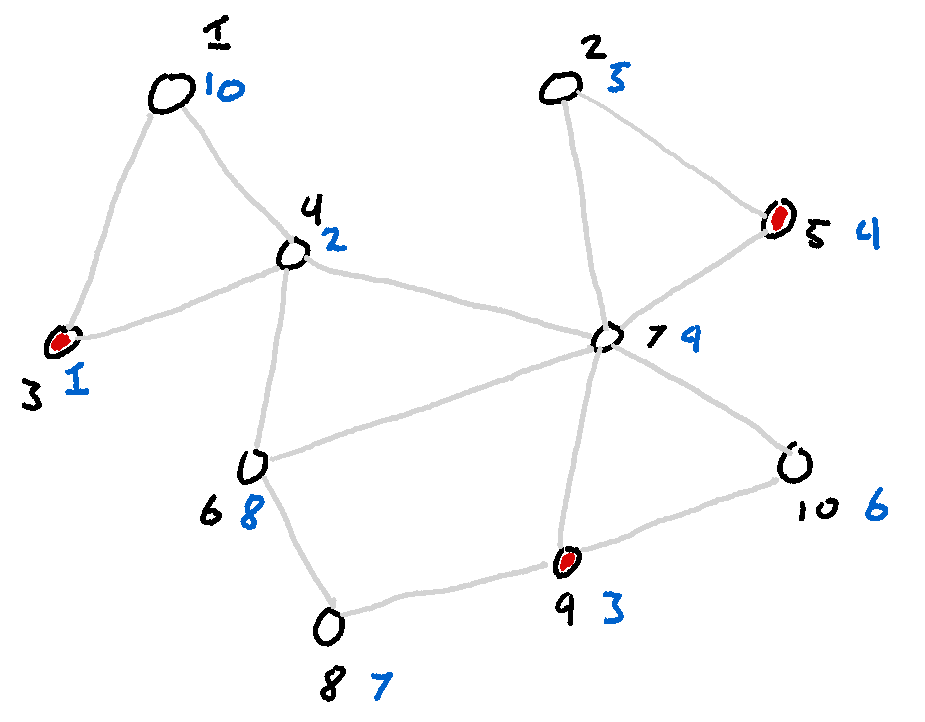
\includegraphics[width = 0.7\textwidth]{graphics/Caro_Wei_construction.png}
            \caption[][0.8cm]{En illustration av vår konstruktion av den oberoende mängden $S$. Vår första etikettering av grafen är i svart, vår ometikettering $\sigma$ i blått, och den resulterande oberoende mängden $S$ markerad i rött.}
        \end{figure}

        Om vi nu låter
        $$S = \left\{i \in V_G \given \sigma(i) < \sigma(j)\quad \forall j \in N(i)\right\}$$
        så hävdar vi att detta måste vara en oberoende mängd. Varför? Tänk för motsägelse att det fanns ett par $i, j$ i $S$ med en kant mellan sig. Eftersom $i$ ligger i $S$ måste alla $i$s grannar ha högre etikett än $i$ -- specifikt så måste alltså $\sigma(i) < \sigma(j)$. Men det betyder ju att $j$ har en granne med lägre etikett, så $j$ kan inte ligga i $S$, och vi har en motsägelse.

        Vi vill alltså förstå oss på mängden $S$. Låt $A_i$ vara händelsen att $i$ fick en lägre etikett än alla sina grannar i vår slumpmässiga ometikettering -- vi har då av väntevärdets linjäritet att
        $$\E{\abs{S}} = \E{\sum_{i=1}^{n} \indSet{A_i}} = \sum_{i=1}^{n} \Prob{A_i}.$$
        
        Det räcker alltså för oss att förstå sannolikheterna för händelserna $A_i$. Eftersom $\sigma$ var likformigt slumpmässig betyder det alltså att vi vill räkna antalet sätt att etikettera grafen sådana att $i$ får en lägre etikett än alla sina grannar.

        För att konstruera ett sådant sätt att etikettera $G$ börjar vi med att välja vilka tal som skall stå på $i$ och dess grannar -- detta kan vi göra på $\binom{n}{d_i + 1}$ sätt, eftersom vi skall ha $d_i$ etiketter på dess grannar och en etikett på den själv.

        Sedan väljer vi hur vi placerar dessa etiketter på $d_i$ och $N(i)$ -- vi måste så klart välja att placera det lägsta av talen på $i$, men de återstående $d_i$ talen kan vi placera ut fritt\sidenote[][]{Det är här som vår teknik med väntevärdets linjäritet verkligen lönar sig -- vi har kunnat zooma in bara på $i$, och behöver inte bry oss om vad som händer utanför just $i$. Hade vi inte gjort det hade vi kanske behövt bekymra oss om kanter mellan $i$s grannar här, och inte kunnat placera ut etiketterna helt fritt.}, och alltså på $d_i!$ sätt.

        Till slut väljer vi hur vi placerar resten av etiketterna på noderna utanför $i$s grannskap -- detta kan vi också göra helt fritt, så på $(n - d_i - 1)!$ sätt. Så totalt har vi sett att det finns
        $$\binom{n}{d_i + 1} d_i! (n - d_i - 1)!$$
        sätt att välja en etikettering av $G$ sådan att $i$ får en lägre etikett än alla sina grannar.

        Så sannolikheten att en slumpmässig etikettering är sådan ges alltså av
        \begin{align*}
            \Prob{A_i} &= \frac{1}{n!}\binom{n}{d_i + 1} d_i! (n - d_i - 1)!\\
            &= \frac{1}{n!}\frac{n!}{(d_i + 1)!(n - (d_i + 1))!}d_i! (n - d_i - 1)!\\
            &= \frac{1}{d_i + 1}
        \end{align*}
        så
        $$\E{\abs{S}} = \sum_{i=1}^{n} \Prob{A_i} = \sum_{i=1}^{n} \frac{1}{d_i + 1}.$$

        Vi har alltså visat att vi \emph{i genomsnitt} hittar en oberoende mängd av vår sökta storlek med denna metoden. Men det genomsnittliga värdet kan ju omöjligen vara mindre än \emph{alla} specifika möjliga värden\sidenote[][-2cm]{
            Låt oss formulera detta som ett lemma och bevisa det:
            \begin{lemma}
                För varje slumpvariabel $X$ med $\E{X} = C$ måste det finnas åtminstone ett $\omega$ sådant att $X(\omega) \geq C$.

                \begin{proof}
                    Antag för motsägelse att $X(\omega) < C$ för alla $\omega$. Då kan vi räkna att
                    \begin{align*}
                        C = \E{X} &= \sum_{\omega \in \Omega} X(\omega)\mu(\omega)\\
                        &< \sum_{\omega \in \Omega} C\mu(\omega)\\
                        &= C\sum_{\omega \in \Omega} \mu(\omega) = C
                    \end{align*}
                    så $C < C$, en motsägelse.
                \end{proof}
            \end{lemma}
        } -- alltså måste det finnas något specifikt val av $\sigma$ sådant att storleken på $S(\sigma)$ blir åtminstone detta. Alltså är vi klara.
    \end{proof}
\end{theorem}

\section{Första-moment-metoden}

Hittills har vi sett ett sätt som väntevärden och sannolikheter kan samspela -- om slumpvariabeln vi vill studera kan formuleras som antalet ``ja'' på en samling ja-nej-frågor så får vi att dess väntevärde är summan av sannolikheterna för ett ``ja'' på varje enskild fråga.

Detta låter oss alltså svara på en fråga om ett väntevärde genom att räkna ut en bunt sannolikheter. Hur gör vi om det vi verkligen är intresserade av är en sannolikhet?

\begin{lemma}[Markovs olikhet]
    Om en icke-negativ\sidenote[][]{Det vill säga, $X(\omega) \geq 0$ för alla $\omega \in \Omega$ -- den tar aldrig ett negativt värde.} slumpvariabel $X$ har väntevärde $\nu$ gäller det för varje $C > 0$ att\sidenote[][]{Eller ekvivalent att
    $$\Prob{X > C} \leq \frac{\nu}{C}.$$}
    $$\Prob{X > C\nu} < \frac{1}{C}.$$

    \begin{proof}
        Vi kan räkna att\sidenote[][]{Var i beviset använder vi antagandet att $X$ är ickenegativ?}
        \begin{align*}
            \nu = \E{X} &= \sum_{\omega \in \Omega} X(\omega)\mu(\omega)\\
            &\geq \sum_{\substack{\omega \in \Omega\\X(\Omega) > C\nu}} X(\omega)\mu(\omega)\\
            &> \sum_{\substack{\omega \in \Omega\\X(\Omega) > C\nu}} C\nu\mu(\omega)\\
            &= C\nu \Prob{X > C\nu}
        \end{align*}
        så om vi delar bägge sidor av detta med $C\nu$ får vi resultatet.
    \end{proof}
\end{lemma}

Vad för slags problem kan man tänkas tillämpa det här verktyget på?

\begin{definition}
    En Erd\H{o}s-Renyi-graf (med parametrar $n$ och $p$) är en slumpmässig graf $G$ på $n$ noder, där varje kant är med med sannolikhet $p$, oberoende av om varje annan kant är med. Vi skriver att $G \sim G_{n,p}$.

    Om $p = \frac{1}{2}$ så kommer alltså $G_{n,p}$ helt enkelt vara en likformigt slumpmässig graf på $n$ noder, men för det mesta kommer vi vara intresserade av fallet när $p$ är en funktion av $n$.
\end{definition}

Vi kan säga en hel del om den ``lokala'' strukturen av en $G_{n,p}$ bara med de verktyg vi har lärt oss hittills -- alltså de egenskaper hos den som vi kan avgöra om de gäller genom att studera den lokalt runt varje nod. Desto svårare blir det om vi ställer oss frågor om ifall den är, till exempel, sammanhängande.

Ett exempel på en lokal struktur är ifall vi har isolerade noder -- om vi tänker oss det som att noderna är personer och kanterna är vänskapsrelationer är vi alltså intresserade av sannolikheten att inte ha några vänner.\sidenote[][-1.1cm]{Som vi alla vet går denna upp markant om man studerar matematik, men vår modell är inte sofistikerad nog att fånga detta.}

\begin{proposition}
    Om $p > \frac{c\log(n)}{n}$ för något $c > 1$ så finns det asymptotiskt nästan säkert\sidenote[][]{Vad sjutton betyder det? Det betyder att, om $p_n$ är en följd sådan att $p_n > \frac{\log(n)}{n}$ för varje $n$, och $G_n$ är en $G_{n, p_n}$ för varje $n$, så går sannolikheten att $G_n$ har en isolerad nod mot noll.} inga isolerade noder\sidenote[][]{Och vad är en isolerad nod? Det är en nod utan grannar.} i $G_{n,p}$.

    \begin{proof}
        Beviset följer ett mönster som förhoppningsvis börjar bli bekant vid det här laget.

        Låt $G \sim G_{n,p}$. Vi låter $I_i$ vara händelsen att nod $i$ är isolerad, och konstaterar att om $I$ är mängden av isolerade noder i $G$ så är
        $$\E{\abs{I}} = \sum_{i=1}^{n} \Prob{I_i}$$
        så vad vi behöver räkna ut är sannolikheten att en viss given nod är isolerad.

        Detta är en relativt enkel beräkning -- det finns $n-1$ noder som $i$ hade kunnat ha en kant till, och varje kant finns med sannolikhet $p$, oberoende av varje annan kant. Alltså är sannolikheten att inga av kanterna finns $(1-p)^{n-1}$, och vi har att
        $$\E{\abs{I}} = \sum_{i=1}^{n} \Prob{I_i} = n(1-p)^{n-1}.$$
        
        Markovs olikhet ger oss nu, för varje $C > 0$, att
        \begin{equation}\label{eq_markov_isolated_verts}
            \Prob{\abs{I} > C\E{\abs{I}}} < \frac{1}{C}.
        \end{equation}

        Hur omvandlar vi detta till det resultat vi vill ha? Om vi tar ett väldigt litet $\epsilon$ och låter $C = \frac{1 - \epsilon}{\E{\abs{I}}}$ så blir \eqref{eq_markov_isolated_verts} till
        $$\Prob{\abs{I} > 1 - \epsilon} < \frac{\E{\abs{I}}}{1 - \epsilon}.$$

        Eftersom $\abs{I}$ självklart enbart tar heltalsvärden är händelsen i vänster led precis samma händelse som händelsen att $\abs{I} \geq 1$, det vill säga $I \neq \emptyset$.\sidenote[][]{Varje tänkbart värde på $\abs{I}$ som är större än $1-\epsilon$ är också $\geq 1$, och vice versa.} Så om vi ersätter vänster led med detta får vi att
        $$\Prob{I \neq \emptyset} < \frac{\E{\abs{I}}}{1-\epsilon}$$
        och här kan vi utan problem ta gränsvärdet $\epsilon \to 0$ och få\sidenote[][]{Notera att vi, när vi tar gränsvärdet här, måste ersätta $<$ med $\leq$ -- för oss är det inget problem eftersom vi oavsett skall visa att $\nu$ går mot noll.}
        $$\Prob{I \neq \emptyset} \leq \E{\abs{I}}.$$

        Så det enda som återstår att göra är att visa att $\E{\abs{I}}$ går mot noll. Enligt satsens antaganden har vi att $p > c\frac{\log(n)}{n}$, så vi kan räkna att
        \begin{align*}
            \lim_{n\to\infty} \E{\abs{I}} &= \lim_{n\to\infty} n(1-p)^{n-1}\\
            &\leq \lim_{n\to\infty} n\left(1 - c\frac{\log(n)}{n}\right)^{n-1}\\
            &= \lim_{n\to\infty} \frac{n}{1 - c\frac{\log(n)}{n}}\left(1 - \frac{c\log(n)}{n}\right)^{n}\\
            &= \lim_{n\to\infty} n\underbrace{\frac{1}{1 - c\frac{\log(n)}{n}}}_{\to\, 1\text{ när }n\,\to\,\infty}\left(\underbrace{\left(1 - \frac{c}{n/\log(n)}\right)^{\frac{n}{\log(n)}}}_{\to\, e^{-c}\text{ när }n\,\to\, \infty}\right)^{\log(n)}\\
            &= \lim_{n \to \infty} n \left(e^{-c}\right)^{\log(n)} = \lim_{n \to \infty} n^{1-c}
        \end{align*}
        och eftersom $c > 1$ går detta mot noll, såsom önskat.\sidenote[][-2.8cm]{I steget mellan rad fyra och fem går vi väldigt snabbt fram -- egentligen hade man behövt kolla att
        $$f(n,c) = \left(1 - \frac{c}{n/\log(n)}\right)^{\frac{n}{\log(n)}}$$
        går mot $e^{-c}$ snabbt nog att vi får lov att göra den substitutionen. Som tur är gäller det att $f(n,c) - e^{-c}$ är ungefär $\frac{\log(n)}{n}$ -- specifikt
        $$\frac{e^{-c} - f(n,c)}{\frac{\log(n)}{n}} \to \frac{c^2}{2e^c}$$
        vilket är bra nog. Men detta är mycket mer analys än vad vi faktiskt vill göra i denna kurs.
        }
    \end{proof}
\end{proposition}

Det finns några saker som är värda att anmärka på här. Om vi hade valt $c \leq 1$ hade inte vår räkning fungerat längre -- och detta är inte ett sammanträffande eller ett resultat av att vi använde en svag metod.

I själva verket kan man visa att antalet isolerade noder faktiskt kommer gå mot oändligheten om $p < \frac{\log(n)}{n}$ -- så vårt resultat är det bästa möjliga.

Vi nämnde innan att vi kan studera lokala problem som dessa enkelt, men att ``globala'' problem är svårare, och nämnde frågan om grafen är sammanhängande som ett exempel på en svår global fråga. I själva verket kan man visa att grafen kommer vara sammanhängande så snart vi inte längre har några isolerade noder -- så detta resultat tillsammans med vad vi just visade visar alltså att en Erd\H{o}s-Renyi-graf är sammanhängande så snart $p \geq \frac{c\log(n)}{n}$.

\section{Räkneregler för slumpvariabler}

Vi sammanfattar vad vi lärt oss om slumpvariabler hittills i följande räkneregler:\sidenote[][]{Den här biten skippar vi på föreläsningen -- den ligger här för att vara behjälplig som sammanfattning och när man gör övningarna. Den finns också i vår samling av formler och räkneregler.}

\begin{lemma}
    Om $(\Omega, \mu)$ är något sannolikhetsrum, $A \subseteq \Omega$ någon händelse, och $X, Y: \Omega \to \R$ samt $Z: \Omega \to V$ är slumpvariabler som tar värden i $\R$ och i någon godtycklig mängd $V$, så gäller att:
    \begin{enumerate}
        \item $$\E{X} = \sum_{x \in X(\Omega)} x \Prob{X = x} = \sum_{\omega \in \Omega} X(\omega)\mu(\omega).$$
        \item För alla $a, b \in \R$ så är
        $$\E{aX + bY} = a\E{X} + b\E{Y}.$$
        Väntevärdet är alltså en linjär funktional.
        \item $$\Prob{A} = \E{\indSet{A}}.$$
        \item Om $X(\omega) \leq C$ för varje $\omega$, eller ekvivalent om $\Prob{X \leq C} = 1$, så är $\E{X} \leq C$.
        \item Om $\E{X} = C$ så finns det åtminstone ett $\omega$ sådant att $X(\omega) \geq C$.
        \item Markovs olikhet ger oss att, om $\E{X_n} \to 0$ för någon följd av ickenegativa slumpvariabler $X_n$ som enbart tar heltalsvärden, så måste också $\Prob{X_n > 0} \to 0$.
        \item Om $Z$ är likformigt fördelad på $V$ så gäller det för varje delmängd $W \subseteq V$ att
        $$\Prob{Z \in W} = \frac{\abs{W}}{\abs{V}}.$$
    \end{enumerate}
\end{lemma}

\section{Övningar}

\begin{xca}
    \begin{definition}
        En familj $\mathcal{F}$ av delmängder till $[n]$ kallas för \emph{skärande} om $A \cap B \neq \emptyset$ för alla par av $A$ och $B$ i $\mathcal{F}$.
    \end{definition}

    Hur stor kan en skärande familj av mängder vara, om vi kräver att varje $A \in \mathcal{F}$ har storlek exakt $k$? Svaret ges av följande sats:

    \begin{theorem}[Erd\H{o}s-Ko-Rado]
        För varje skärande familj $\mathcal{F}$ av delmängder av storlek $k$ till $[n]$ gäller det att
        $$\abs{F} \leq \binom{n-1}{k-1}.$$
    \end{theorem}

    \textbf{Delfråga a:} Hitta, för alla $n$ och $k$, ett exempel på en skärande familj $\mathcal{F}$ av delmängder av storlek $k$ till $[n]$ sådan att
    $$\abs{F} \leq \binom{n-1}{k-1}.$$

    \textbf{Delfråga b:} Bevisa följande lemma:\sidenote[][]{Den här delen kräver ingen probabilistisk metod, det är bara ett direkt bevis. Sannolikhetsteorin kommer in i nästa delfråga.}

    \begin{lemma}
        Låt $\mathcal{F} \subseteq \binom{[n]}{k}$ vara en skärande familj, och låt för varje $s \in \{0,1,\ldots,n-1\}$
        $$A_s = \{s, s+1, \ldots, s + k - 1\}$$
        där additionen är modulo $n$. Då kan $\mathcal{F}$ innehålla högst $k$ av mängderna $A_s$.
    \end{lemma}

    Dra sedan slutsatsen från detta att samma lemma gäller även om vi tar någon permutation $\sigma \in S_n$ och låter
    $$A_s = \{\sigma(s), \sigma(s+1), \ldots, \sigma(s + k - 1)\}.$$

    \textbf{Delfråga c:} Nu skall vi bevisa Erd\H{o}s-Ko-Rado. Idén är att vi vill skapa en likformigt slumpmässig $A \uniformIn \binom{[n]}{k}$ och studera sannolikheten att denna ligger i $\mathcal{F}$ -- det finns ett uppenbart uttryck för denna sannolikhet, och vi vill skapa $A$ på ett sätt som gör att vi också kan använda vårt lemma från förra delfrågan för att begränsa den.

    Beviset börjar alltså med ``Tag en likformigt fördelad permutation $\sigma \uniformIn S_n$ och ett likformigt fördelat heltal $s \uniformIn \{0,1,\ldots,n-1\}$''. Skriv resten av beviset.
\end{xca}

\begin{xca}
    Bevisa följande proposition:

    \begin{proposition}
        Antag att $v_1, v_2, \ldots, v_n$ är $n$ stycken enhetsvektorer i $\R^n$, alltså $\norm{v_i} = 1$ för alla $i$. Då finns det en följd $\eta_1, \eta_2, \ldots, \eta_n$, med $\eta_i = \pm 1$ för varje $i$, sådan att
        $$\norm{\sum_{i=1}^{n} \eta_i v_i} \leq \sqrt{n}.$$
    \end{proposition}
\end{xca}

\begin{xca}
    I denna övning skall vi bevisa följande resultat:

    \begin{theorem}
        Låt $G = (V, E)$ vara någon graf, och antag att $\abs{V} = n$ och $\abs{E} = n\frac{d}{2}$ för något $d \geq 1$. Då finns det en oberoende mängd i $G$ av storlek åtminstone $\frac{n}{2d}$.
    \end{theorem}

    Idén för beviset är att vi tar en slumpmässig delmängd $S \subseteq V$ genom att ta med varje nod med sannolikhet $p = \frac{1}{d}$. Denna kommer så klart inte vara garanterad att vara en oberoende mängd -- men om vi, för varje kant $\{u, v\}$ som kopplar ihop $u, v \in S$ , tar bort $u$ eller $v$ ur $S$ så blir den återstående mängden av noder oberoende.

    Bevisa satsen genom att räkna ut väntevärdet av storleken på $S$ och väntevärdet av antalet noder vi tvingas ta bort ur $S$, och se att vi kommer ha i genomsnitt $\frac{n}{2d}$ noder kvar.
\end{xca}

\begin{xca}
    Låt $p \in (0,1)$ vara fixt. För varje $i \in \N$, låt 
    $$X_i = \begin{cases}
        1  & \text{med sannolikhet }p\\
        0 & \text{annars},
    \end{cases}$$
    så att $X_1, X_2, X_3, \ldots$ blir en slumpmässig följd av nollor och ettor. Låt $I$ vara det minsta $I$ sådant att $X_I = 0$ -- detta blir alltså ett slumpmässigt heltal.

    Beräkna, för varje $i \in \N$, $\Prob{I = i}$. Räkna sedan ut $\E{I}$.
\end{xca}

\begin{xca}
    Antag att du samlar på Pokemonkort.\sidenote[][]{Ersätt med ditt favorit-gacha med lootboxes om du vill ha ett mer samtida exempel.} Vi föreställer oss en väldigt enkel modell för hur du får ett nytt kort -- det finns $n$ stycken distinkta kort totalt, och du kan köpa ett nytt kort åt taget. Det nya kortet du får är likformigt fördelat i samlingen av kort -- varje kort är lika sannolikt.

    När du köper ditt första kort är du garanterad att få ett kort du inte har innan. När du köper ditt andra kort är sannolikheten bara $\frac{1}{n}$ att du råkar få det kort du redan fick en gång -- men när du redan har de flesta av korten kommer du oftast bara att få ett kort du redan äger, inte ett nytt, så du behöver köpa väldigt många paket för att gå från att ha en samling av $n-1$ kort till att ha en fullständig samling.

    Låt $T$ vara antalet gånger du behöver köpa ett nytt kort för att få en fullständig samling, om du börjar på noll. Beräkna $\E{T}$.\sidenote[][]{Ledtråd: Lösningen på det här problemet använder lösningen på föregående problem.}
\end{xca}

\begin{xca}
    Använd väntevärdets linjäritet för att ge ytterligare ett alternativt bevis för unionsbegränsningen.\sidenote[][]{Ledtråd: Återigen algebra med indikatorvariabler. Hur uttrycker man $\ind{A \cup B}$ i termer av $\ind{A}$ och $\ind{B}$?}
\end{xca}

%\bibliography{references}
%\bibliographystyle{plainnat}

\end{document}
